\newpage
\section{Umsetzung (ca. 10 Seiten)}
Nachdem die theoretischen Grundlagen im letzten Kapitel vorgestellt wurden, wird in diesem Kapitel die Umsetzung beschrieben. Dieses Kapitel wird nach einem geordneten Vorgehen strukturiert. Zuerst werden verfügbare Daten vorgestellt, analysiert und sortiert. In diesem Schritt wird entschieden, welche Daten die Zielvariable Nachfrage beeinflussen und somit mit in das Modell eingegeben werden. Die deskriptive Analyse unterstützt dabei die Visualisierung der Daten und verleiht mehr Verständnis für den Ablauf der Media-Kanäle. Darauffolgend werden die Daten in das OLS-Modell eingesetzt. Die Ergebnisse des Modells werden analysiert.
\subsection{Einsatz der deskriptiven Analyse für die Datenbewertung}
Wie im \autoref{deskriptiveanalyse} beschrieben, fasst die deskriptive Analyse historische Daten zusammen und zeigt wichtige Muster und Trends auf. Sie bildet die Grundlage für weiterführende Analysen und datengestützte Entscheidungen. Um auf den Einsatz des \ac{OLS}-Modells vorzubereiten, werden die Daten vom \ac{MMM} deskriptiv analysiert. \\\\
Für das \ac{MMM}-Modell (s. \autoref{fig:mmmbonprix}) stehen Daten vom 01.01.2022 bis 01.01.2024 zur Verfügung. Diese Daten umfassen die Marketing-Ausgaben, wie Katalogausgaben, Online-Marketingausgaben und Mediaausgaben. Für Mediakanäle sind spezifisch auch die Kosten der Unterkanäle dabei. 
Unter diesen Daten fallen auch Kosten für (adressierbares) TV, Podcasts, \ac{dooh}+\ac{ooh}, Radio, YouTube, soziale Medien, Online-Videos und Display-Medien. Für die internen Faktoren sind Kosten von E-Mail, Push-Nachrichten und Verkaufsförderungen wie Versandkostenbefreiung und Rabatt verfügbar. Für die externen Faktoren ist ein Saisonalitätswert von einem Facebook-Saisonmodell vorhanden. Um die Wettbewerber im Modell zu berücksichtigen, sind auch Marketingausgaben von C\&A, H\&M, About You und Zalando verfügbar. Zum Schluss ermöglichen Nachfrage und Datum, den Verlauf sowie die Auswirkungen aller Faktoren auf Tagesbasis darzustellen. \\\\
Da es auf der Media-Ebene modelliert wird, werden nicht alle Daten von dem \ac{MMM} benötigt. Für den Anfang werden nur für Media relevante Daten für das Modell entnommen. Die Daten werden von der Google BigQuery Cloud in die Google Jupyter-Notebook-Instanz geladen, um dort mit Python modelliert zu werden. Die Daten bilden eine Tabelle, in der jede Zeile nach Datum sortiert ist und einen Tag mit den Informationen aller Variablen darstellt. \\\\
Zuerst wird die Qualität der Daten für das \ac{MMM} überprüft. Wie im \autoref{methodederkleinstenquadrate} beschrieben, führen Redundanzen zu einem falschen Ergebnis im Modell. Deshalb soll es überprüft werden, ob es allgemein Redundanzen in den Zeilen gibt. Auch ohne \(y_i\) kann der Koeffizient $\beta$ nicht geschätzt werden. In dem Media-Modell ist die Nachfrage der Zielwert \(y_i\), da es gerechnet werden soll, wie viel ein Euro als Ausgabe in einem Media-Kanal in der Nachfrage bringt. Die Nachfrage darf deswegen nicht Null sein. Daher wird im ersten Schritt überprüft, ob allgemein Redundanzen vorliegen und ob in der Spalte \anf{demand} Nullwerte vorhanden sind.\\\\
So wurde der Code \verb|df_raw[df_raw['demand'].isnull()]| ausgeführt, um Zeilen mit einem leeren Nachfrage-Wert abzufragen. Dabei wurde eine Zeile mit einem leeren Nachfrage-Wert am 29.06.2024 identifiziert. Um den Null-Wert zu korrigieren, wurde der Durchschnitt der Nachfragen am 28.06.2024 und am 30.06.2024 für das Datum 29.06.2024 berechnet.  
\begin{lstlisting}[language=Python, linewidth=\textwidth]
mask = (df_raw['date'] == '2024-06-29')
avg_demand = df_raw.loc[df_raw['date'].isin(['2024-06-28', '2024-06-30']), 'demand'].mean()
df_raw.loc[mask, 'demand'] = avg_demand
\end{lstlisting}


\begin{figure}[ht]
    \centering
    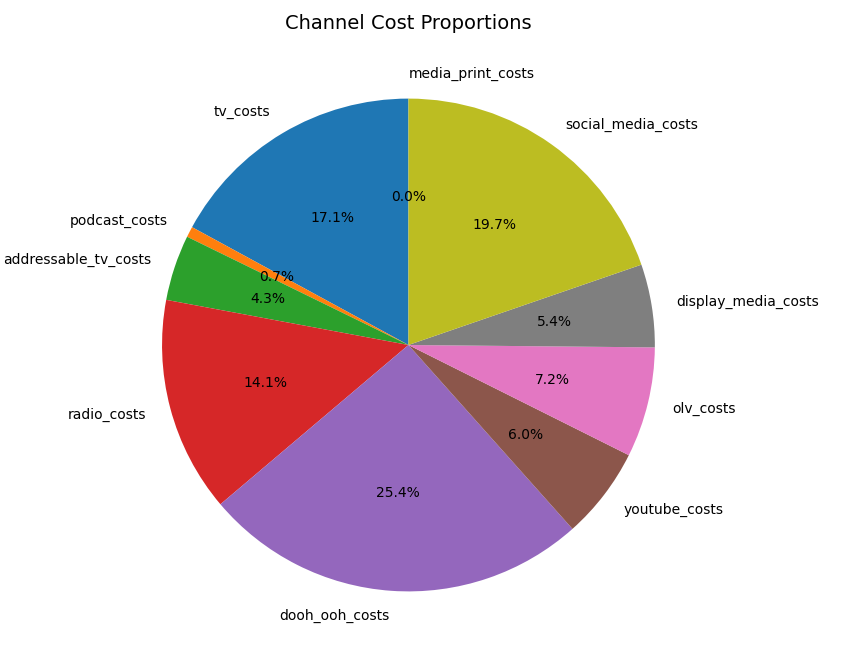
\includegraphics[width=0.8\linewidth]{images/mediapie.png}
    \caption{Kostenanteil der Media-Kanäle bei bonprix, eigene Darstellung}
    \label{fig:mediapie}
\end{figure}

\subsection{Daten auswerten}
\subsection{Einsetzung des Marketing-Mix-Modells}
\subsection{Modell-Ergebnis}
